\chapter{Testing}
\label{testing}
\section{Setup}
In order to ensure \tool\ fulfills the requirements stated in Chapter~\ref{introduction} we performed several tests.
To be able to check the results for correctness, we kept the testing network small and simple.
The layout of the test setup can be seen in Figure~\ref{fig:test_setup}.
While a very basic network, it is sufficient for the tests described below, which will guarantee the required capabilities of \tool.
We changed the priority of bridge \textit{C} to 61440 (the maximum) to ensure it would not be root.
For bridges \textit{A} and \textit{B} we used the systemd id extension to ensure they would not be root when our \textit{Root} bridge was connected.
Nodes \textit{A}, \textit{B} and \textit{C} were running \textit{Wireshark} and \tool.
Additionally using \textit{Wireshark} allowed us to check the actual packages involved in the testing process to monitor progress and note situations not handled correctly by \tool.
The server for \tool\ was run on Node \textit{C}.
Test results were checked for their correctness by checking the report provided by \tool\ against the layout the network actually has.
This layout was deduced using the debug output from our running \textit{software-switch} instances and the configuration of the hardware switches.

\begin{figure}[h]
    \begin{center}
        \begin{subfigure}[b]{0.4\textwidth}
            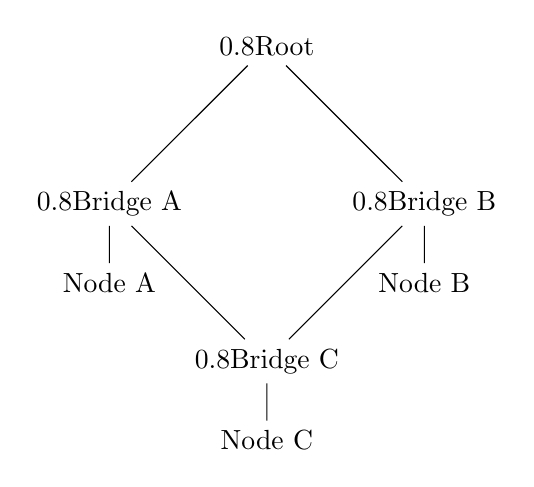
\begin{tikzpicture}
                \node (root) at (2, 4) {\switch{0.8}{Root}};
                \node (a) at (0, 2) {\switch{0.8}{Bridge A}};
                \node (na) at (0, 1) {Node A};
                \node (b) at (4, 2) {\switch{0.8}{Bridge B}};
                \node (nb) at (4, 1) {Node B};
                \node (c) at (2, 0) {\switch{0.8}{Bridge C}};
                \node (nc) at (2, -1) {Node C};
                \draw 
                (root) -- (a)
                (root) -- (b)
                (a) -- (c)
                (b) -- (c)
                (a) -- (na)
                (b) -- (nb)
                (c) -- (nc);
            \end{tikzpicture}
            \caption{Test setup}
            \label{fig:test_setup1}
        \end{subfigure}
        \hspace{1cm}
        \begin{subfigure}[b]{0.4\textwidth}
            \centering
            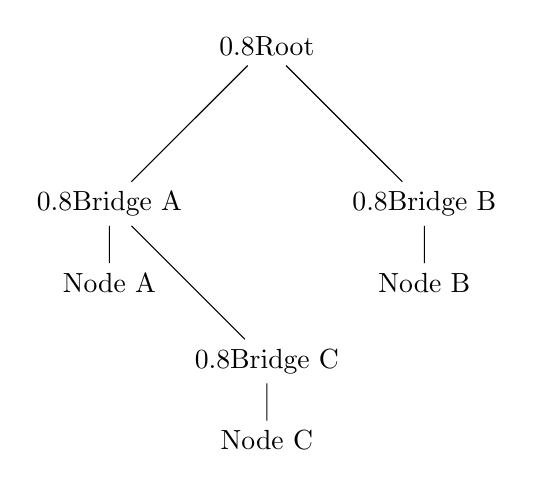
\begin{tikzpicture}
                \node (root) at (2, 4) {\switch{0.8}{Root}};
                \node (a) at (0, 2) {\switch{0.8}{Bridge A}};
                \node (na) at (0, 1) {Node A};
                \node (b) at (4, 2) {\switch{0.8}{Bridge B}};
                \node (nb) at (4, 1) {Node B};
                \node (c) at (2, 0) {\switch{0.8}{Bridge C}};
                \node (nc) at (2, -1) {Node C};
                \draw 
                (root) -- (a)
                (root) -- (b)
                (a) -- (c)
                (a) -- (na)
                (b) -- (nb)
                (c) -- (nc);
            \end{tikzpicture}
            \caption{Expected STP overlay}
            \label{fig:test_setup2}
        \end{subfigure}
    \end{center}
    \caption{The expected physical and logical network topologies}
    \label{fig:test_setup}
\end{figure}

\subsection*{Actual Physical Setup}
\label{physical_setup}
Due to our problems with \textit{OpenWrt} and \textit{dd-wrt} we had to use our \textit{software-switch} tool for testing.
We ran it on two laptops, which were bridges \textit{A} and \textit{B}.
USB to Ethernet adapters were used to give the laptops an additional Ethernet port and make them usable.
To reduce the amount of ports we needed, we ran \tool\ instances on the laptops themselves instead of on a seperate node.
Unfortunately, the laptop replacing bridge \textit{B} sometimes got confused which interface to use for the default route when all interfaces were connected.
This stopped it from sending data to the server, which caused the server to remove all its old data.
It is not an issue with anything we developed, but rather \textit{NetworkManager} running on the laptop.
The tests were not really affected, as whether bridge \textit{A} was contained in the visualization was irrelevant in the cases where it happened.
We decided no to set the timeout in the server to a large number to circumvent this, because this might have interfered with the actual test we wanted to perform.

In an actual scenario, where \tool\ is running on a seperate device, this is not an issue.
Not even if some of the bridges in the network were running our \textit{software-switch} utility, as basic switching was tested and is functional.

The devices we used have the following bridge IDs:
\begin{itemize}
    \item \textbf{Root Bridge}: BC:AE:C5:EB:7D:B6
    \item \textbf{Bridge A}: 00:E0:7C:C8:57:E7
    \item \textbf{Bridge B}: 00:E1:00:00:0D:C4
    \item \textbf{Bridge C}: F4:F2:6D:7D:BF:BD
\end{itemize}

\section{Tests}
\subsection*{"Plug and Play" Test}
\label{usage_test}
This test is meant to ensure the general bridge discovery ability of \tool.
It is designed to simulate the connection of nodes to an established network.
Using a simple setup like shown in Figure~\ref{fig:test_setup1} allows us to collect information about the whole network.
If we were using less nodes than we had non-root bridges in the network, this would not be possible.

\subsubsection*{Performing the test}
\begin{enumerate}
    \item The layout shown in Figure~\ref{fig:test_setup1} was established and all devices were started.
    \item No \tool\ instance was started yet, identification during the tree establishment is covered by Section~\ref{tree_est_test}: Tree Establishment Test.
    \item We waited for the bridges to establish a stable spanning tree, checking the progress by observing the STP packets for the TC flag.
    \item After the tree had stabilized we started the server on node \textit{A}, as well as \tool\ on all the nodes.
    \item We waited for the \tool\ instances to send their data to the server, which takes one $helloTime$ plus the latency between the nodes and the server.
    \item When all nodes had sent their data to the server we created a report to check it against the expected result.
\end{enumerate}
\subsubsection*{Expected Result}
With the limited size of the test network all bridges can and must be identified correctly for this test to be counted as successful.
If the bridges in the network behave as they should, \tool\ should not be able to gather information about connections between the bridges.
Figure~\ref{fig:pnpExp} shows the output we expect.

\subsubsection*{\tool\ Output}
All nodes are correctly identified.
As the tree is already established when \tool\ is started on all nodes, no information about connections between the bridges can be gathered.
Figure~\ref{fig:pnp} shows a comparison between expected output ant \tool\ output.
\begin{figure}[h]
    \begin{subfigure}[b]{\textwidth}
        \centering
        \begin{tikzpicture}
            \node (root) at (2, 4) {\switch{0.8}{Root}};
            \node (a) at (0, 2) {\switch{0.8}{A}};
            \node (b) at (2, 2) {\switch{0.8}{B}};
            \node (empty) at (4, 2) {};
            \node (c) at (4, 0) {\switch{0.8}{C}};

            \draw
            (root) -- (a)
            (root) -- (b)
            (root) -- (empty)
            (empty) -- (c);

        \end{tikzpicture}
        \caption{Expected result}
        \label{fig:pnpExp}
    \end{subfigure}
    
    \vspace{0.5cm}

    \begin{subfigure}[b]{\textwidth}
        \centering
        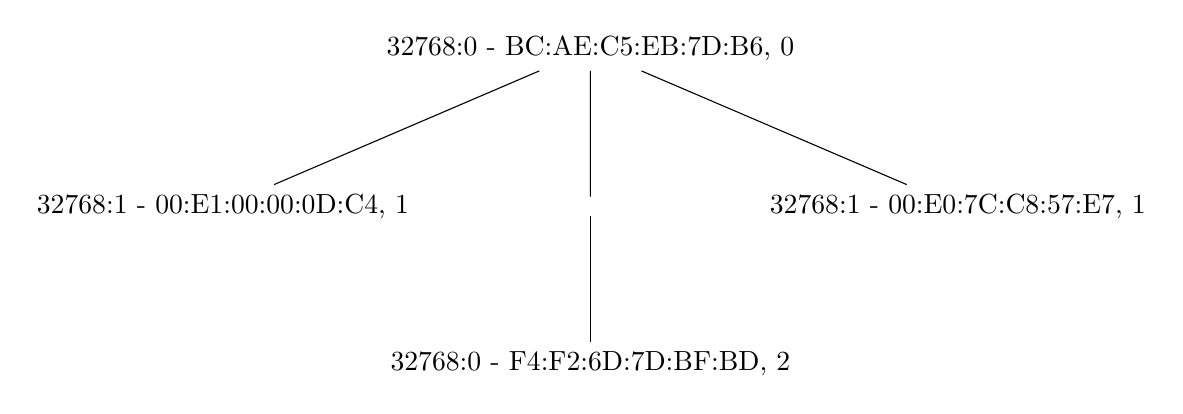
\begin{tikzpicture}[]
\node (0) at (7.000000,20) {32768:0 - BC:AE:C5:EB:7D:B6, 0};
\node (1) at (2.333333,18) {32768:1 - 00:E1:00:00:0D:C4, 1};
\node (2) at (7.000000,18) {};
\node (3) at (7.000000,16) {32768:0 - F4:F2:6D:7D:BF:BD, 2};
\draw (2) -- (3);
\node (4) at (11.666667,18) {32768:1 - 00:E0:7C:C8:57:E7, 1};
\draw 
(0) -- (1)
(0) -- (2)
(0) -- (4);
\end{tikzpicture}

        \caption{\tool\ output}
    \end{subfigure}
    \caption{Expected output compared to \tool\ output ("Plug and Play" Test)}
    \label{fig:pnp}
\end{figure}

\subsection*{Tree Establishment Test}
\label{tree_est_test}
To test whether \tool\ can handle bridges being added to the network during runtime, we start \tool\ on all nodes before the establishment of the spanning tree, and check for correct identification afterwards.

\subsubsection*{Performing the test}
\begin{enumerate}
    \item The layout shown in Figure~\ref{fig:test_setup} was established and all devices were started.
    \item Before enabling STP on all the bridges we started the server and \tool\ instances.
    \item After enabling STP on the bridges we waited for the tree to be established, again checking the progress via the TC flag.
    \item Finally we checked the result for correctness.
\end{enumerate}

\subsubsection*{Expected Result}
Again all the bridges can and must be correctly identified.
Additionally, this time the identification of bridge connections is possible, and the topology should therefore be fully identified.

\subsubsection*{\tool\ Output}
If bridge \textit{D} is connected to bridges \textit{B} and \textit{C} before they are connected to bridge \textit{A}, the tree can build up slowly and the clients will know about the connections.
The resulting visualization can be seen in Figure~\ref{fig:est}
\begin{figure}[h]
    \begin{subfigure}[b]{\textwidth}
        \centering
            \begin{tikzpicture}
                \node (root) at (2, 4) {\switch{0.8}{Root}};
                \node (a) at (0, 2) {\switch{0.8}{A}};
                \node (b) at (4, 2) {\switch{0.8}{B}};
                \node (c) at (2, 0) {\switch{0.8}{C}};

                \draw
                (root) -- (a)
                (root) -- (b)
                (a) -- (c);
            \end{tikzpicture}
            \caption{Expected result}
    \end{subfigure}

    \vspace{0.5cm}

    \begin{subfigure}[b]{\textwidth}
        \centering
        \input{../results/estWorking.tikz}
        \caption{\tool\ output}
    \end{subfigure}
    \caption{The result of the Tree Establishment Test}
    \label{fig:est}
\end{figure}

\subsection*{Bridge Removal Test}
\label{removal_test}
\tool\ must also be able to react to bridges or clients dropping from a network.
This test makes sure that capability is given.

\subsubsection*{Performing the test}
\begin{enumerate}
    \item We started all the nodes \tool\ instances and waited for the spanning tree to be established and correctly identified (see the sections on the Usage Test \ref{usage_test} and the Tree Establishment Test \ref{tree_est_test}).
    \item After the tree was constructed we unplugged Node \textit{A} and waited for the tree to stabilize.
    \item Finally we checked the output of the report for correct identification of the smaller tree.
\end{enumerate}

\subsubsection*{Expected Result}
Bridge \textit{A} must correctly be removed from the topology visualization.
The expected topology is shown in Figure~\ref{fig:removalExp}.

\subsubsection*{\tool\ Output}
As visible in Figure~\ref{fig:removal}, the bridge is correctly removed.
This is one of the cases where the laptop running bridge \textit{B} stopped sending data to the server.
The removal of bridge \textit{A} is still visible however, and so we deemed this test successful.

\begin{figure}[h]
    \begin{subfigure}[b]{\textwidth}
        \centering
        \begin{tikzpicture}[]
            \node (root) at (2,4) {\switch{0.8}{Root}};
            \node (empty) at (0, 2) {};
            \node (c) at (0,0) {\switch{0.8}{C}};
            \node (b) at (4,2) {\switch{0.8}{B}};

            \draw
            (root) -- (empty)
            (root) -- (b)
            (empty) -- (c);
        \end{tikzpicture}
        \caption{The expected result}
        \label{fig:removalExp}
    \end{subfigure}

    \vspace{0.5cm}

    \begin{subfigure}[b]{\textwidth}
        \centering
        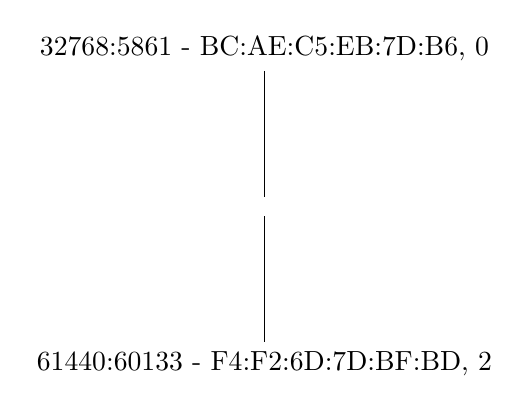
\begin{tikzpicture}[]
\node (0) at (7.000000,20) {32768:5861 - BC:AE:C5:EB:7D:B6, 0};
\node (1) at (7.000000,18) {};
\node (2) at (7.000000,16) {61440:60133 - F4:F2:6D:7D:BF:BD, 2};
\draw (1) -- (2);
\draw 
(0) -- (1);
\end{tikzpicture}
        \caption{The \tool\ output}
    \end{subfigure}
    \caption{Expected output compared to \tool\ output (Tree Removal Test)}
    \label{fig:removal}
\end{figure}

\subsection*{Slow Dynamic Change Test}
\label{slow_dynamic_test}
Changes in the network topology must not be a problem for \tool.
By successfully testing for additions and removals from the network (Section~\ref{usage_test}: "Plug and Play" test and Section~\ref{removal_test}: Removal Test) one could assume that changes can be handled as well, but caution demands that we test specifically for changes in the topology.
Due to the rather complex nature of this test, Figure~\ref{fig:sdcTest} shows the physical network topology after every step.

\subsubsection*{Performing the test}
\begin{enumerate}
    \item We set up all the nodes and waited for a stable tree to be generated by the bridges like before.
    \item We disconnected bridge \textit{A} from the root, resulting in a topolgy like in Figure~\ref{fig:sdcTest2}.
    \item The connection between bridges \textit{B} and \textit{C} was also severed, leaving bridges \textit{A} and \textit{C} in a disconnected subtree, as shown in Figure~\ref{fig:sdcTest3}.
    \item We waited for the spanning tree to stabilize after the removal.
    \item Bridges \textit{A} and \textit{C} were connected to bridge \textit{B} yielding the physical topology shown in Figure~\ref{fig:sdcTest5}.
    \item After the tree had stabilized we checked the report output for correctness.
\end{enumerate}

\begin{figure}[h]
    \begin{center}
        \begin{subfigure}[b]{0.4\textwidth}
            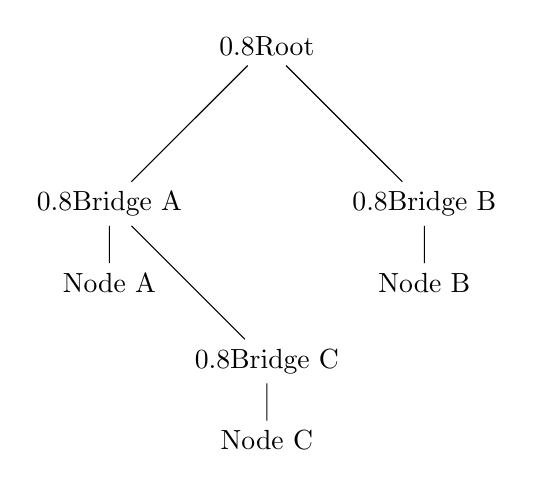
\begin{tikzpicture}
                \node (root) at (2, 4) {\switch{0.8}{Root}};
                \node (a) at (0, 2) {\switch{0.8}{Bridge A}};
                \node (na) at (0, 1) {Node A};
                \node (b) at (4, 2) {\switch{0.8}{Bridge B}};
                \node (nb) at (4, 1) {Node B};
                \node (c) at (2, 0) {\switch{0.8}{Bridge C}};
                \node (nc) at (2, -1) {Node C};
                \draw 
                (root) -- (a)
                (root) -- (b)
                (a) -- (c)
                (a) -- (na)
                (b) -- (nb)
                (c) -- (nc);
            \end{tikzpicture}
            \caption{The topology before the test}
        \end{subfigure}
        \hspace{1cm}
        \begin{subfigure}[b]{0.4\textwidth}
            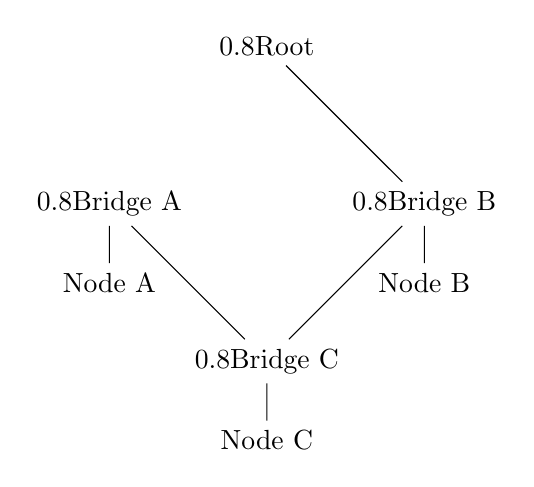
\begin{tikzpicture}
                \node (root) at (2, 4) {\switch{0.8}{Root}};
                \node (a) at (0, 2) {\switch{0.8}{Bridge A}};
                \node (na) at (0, 1) {Node A};
                \node (b) at (4, 2) {\switch{0.8}{Bridge B}};
                \node (nb) at (4, 1) {Node B};
                \node (c) at (2, 0) {\switch{0.8}{Bridge C}};
                \node (nc) at (2, -1) {Node C};

                \draw
                (root) -- (b)
                (b) -- (nb)
                (b) -- (c)
                (a) -- (c)
                (a) -- (na)
                (c) -- (nc);
            \end{tikzpicture}
            \caption{The topology after step 2}
            \label{fig:sdcTest2}
        \end{subfigure}

    \end{center}
    \begin{center}
        \begin{subfigure}[b]{0.4\textwidth}
            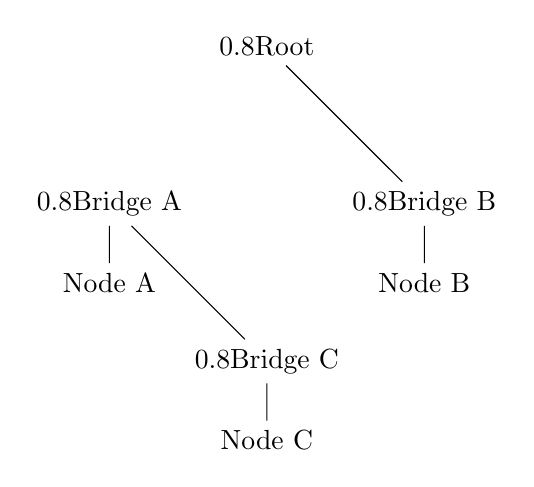
\begin{tikzpicture}
                \node (root) at (2, 4) {\switch{0.8}{Root}};
                \node (a) at (0, 2) {\switch{0.8}{Bridge A}};
                \node (na) at (0, 1) {Node A};
                \node (b) at (4, 2) {\switch{0.8}{Bridge B}};
                \node (nb) at (4, 1) {Node B};
                \node (c) at (2, 0) {\switch{0.8}{Bridge C}};
                \node (nc) at (2, -1) {Node C};

                \draw
                (root) -- (b)
                (b) -- (nb)
                (a) -- (c)
                (a) -- (na)
                (c) -- (nc);
            \end{tikzpicture}
            \caption{The topology after subtree removal}
            \label{fig:sdcTest3}
        \end{subfigure}
        \hspace{1cm}
        \begin{subfigure}[b]{0.4\textwidth}
            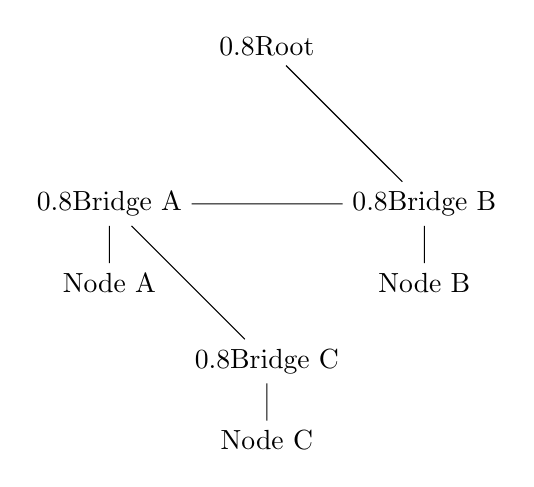
\begin{tikzpicture}
                \node (root) at (2, 4) {\switch{0.8}{Root}};
                \node (a) at (0, 2) {\switch{0.8}{Bridge A}};
                \node (na) at (0, 1) {Node A};
                \node (b) at (4, 2) {\switch{0.8}{Bridge B}};
                \node (nb) at (4, 1) {Node B};
                \node (c) at (2, 0) {\switch{0.8}{Bridge C}};
                \node (nc) at (2, -1) {Node C};

                \draw 
                (root) -- (b)
                (b) -- (a)
                (a) -- (c)
                (a) -- (na)
                (b) -- (nb)
                (c) -- (nc);
            \end{tikzpicture}
            \caption{The topology after the test}
            \label{fig:sdcTest5}
       \end{subfigure}
    \end{center}
    \caption{The physical topology during the Slow Dynamic Test}
    \label{fig:sdcTest}
\end{figure}

\subsubsection*{Expected Result}
Because we wait for the small subtree to stabilize, establishing bridge \textit{A} as root, the subtree should be correctly identified, with the connection between the bridges.
Bridge \textit{A} should not be connected to this subtree in the output, as the \textit{Root} bridge should be recognized immediately on reconnecting.

\subsubsection*{\tool\ Output}
During the test we checked the server output to see how disconnecting the two clients affected the output.
We were surprised to see that it had not changed.
After checking the \textit{Wireshark} output, we realized that this was because no TC flag had been sent.
Figure~\ref{fig:noTc} shows the packet capture, including the changed packets.
We marked the line after which the root identifier is updated.
Where it should say \textit{Conf. + TC} (meaning a configuration packet with set TC flag), a regular configuration packet was indicated.
\begin{figure}[h]
    \centering
    \includegraphics[width=0.8\textwidth]{noTc.png}
    \caption{The packet capture not showing a TC flag}
    \label{fig:noTc}
\end{figure}

As we realized during earlier testing, the TC flag is not always sent when a change occurs.
This is why the client also looks for changes in message ages and the bridges in the STP packet.
Due to the message age decreasing (one of the bridges is now root), the client will clear its data even without a TC flag.
With the subtree stabilized, the client will prepend the \textit{Root} bridge to \textit{A} and \textit{C} on reconnection. 

The visualization acquired before executing the test is the same as in Figure~\ref{fig:est}, as we used that test as preparation.
Unfortunately, bridge \textit{B} stopped sending again.
However, the test was a success, as the subtree was correctly identified and added to the large tree.
The visualization we obtained from \tool can be seen in Figure~\ref{fig:dynAfter}.
\begin{figure}[h]
    \begin{subfigure}[b]{\textwidth}
        \centering
        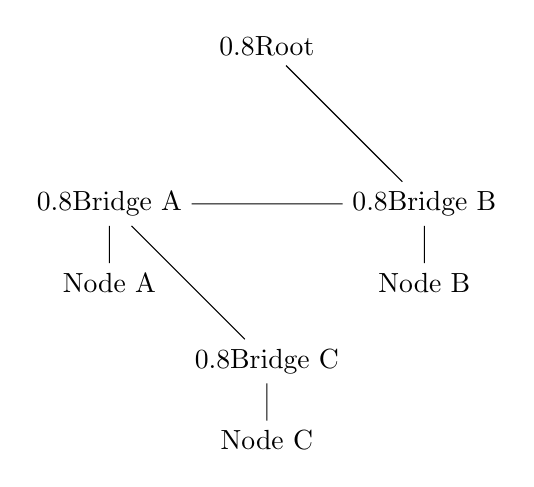
\begin{tikzpicture}
            \node (root) at (2, 4) {\switch{0.8}{Root}};
            \node (a) at (0, 2) {\switch{0.8}{Bridge A}};
            \node (na) at (0, 1) {Node A};
            \node (b) at (4, 2) {\switch{0.8}{Bridge B}};
            \node (nb) at (4, 1) {Node B};
            \node (c) at (2, 0) {\switch{0.8}{Bridge C}};
            \node (nc) at (2, -1) {Node C};

            \draw 
            (root) -- (b)
            (b) -- (a)
            (a) -- (c)
            (a) -- (na)
            (b) -- (nb)
            (c) -- (nc);
        \end{tikzpicture}
        \caption{The expected result}
    \end{subfigure}
       
    \vspace{0.5cm}

    \begin{subfigure}[b]{\textwidth}
        \centering
        \begin{tikzpicture}[]
\node (0) at (7.000000,20) {32768:5861 - BC:AE:C5:EB:7D:B6, 0};
\node (1) at (3.500000,18) {};
\node (2) at (3.500000,16) {};
\node (3) at (3.500000,14) {61440:39025 - F4:F2:6D:7D:BF:BD, 3};
\draw (2) -- (3);
\draw (1) -- (2);
\node (4) at (10.500000,18) {};
\node (5) at (10.500000,16) {32768:39025 - 00:E0:7C:C8:57:E7, 2};
\draw (4) -- (5);
\draw 
(0) -- (1)
(0) -- (4);
\end{tikzpicture}
        \caption{\tool\ output}
    \end{subfigure}
    \caption{Expected output compared to \tool\ output (Slow/Fast Dynamic Change Test)}
    \label{fig:dynAfter}
\end{figure}

\subsection*{Fast Dynamic Change Test}
\label{fast_dynamic_test}
Robustness to changes in the topology are a must for \tool.
It would however also be nice if \tool\ were robust enough to handle topology changes without a spanning tree stabilization in between.
The logical topology is the same as for the Slow Dynamic Change Test \ref{slow_dynamic_test}

\subsubsection*{Performing the test}
The steps required to perform this test are the same as for Section~\ref{slow_dynamic_test}: Slow Dynamic Test, with one difference.
This time we did not wait for the subtree to stabilize (after Figure~\ref{fig:sdcTest3}), but instead immediately plugged bridge \textit{A} into bridge \textit{B}.

\subsubsection*{Expected Result}
We did not know what to expect.
The nodes should be correctly identified, but we were unsure about the connections, as it was not clear how each bridge would update.

\subsubsection*{\tool\ Output}
For the first few seconds after reconnecting the subtree to bridge \textit{B} (Figure~\ref{fig:sdcTest5}) nothing happened.
After that, the bridges updated their information, which resulted in the same visualization as the Slow Dynamic Change Test.
This means that our approach to keeping and saving bridge connection data is stable enough to withstand sudden topology changes.
The output is identical to Figure~\ref{fig:dynAfter}.
